\chapter{THEORETICAL FRAMEWORK}

This chapter aims to introduce key definitions and theoretical foundations across interconnected areas that underpin this research: (1) spatio-temporal data representation and analysis, (2) large language models and their architectural principles, (3) fine-tuning and adaptation techniques, (4) prompting strategies, (5) tool-integrated reasoning approaches, and (6) evaluation metrics. These foundational concepts collectively establish the theoretical basis required to comprehend the approaches and methodologies employed throughout this work.

\section{Spatio-Temporal Data}

The spatio-temporal data is a type of data that contains information about the spatial and temporal dimensions of an event or phenomenon. 
This dual indexing enables the representation of complex relationships between spatial and temporal elements, allowing for a more comprehensive understanding of the data.

The spatio-temporal data can be formalized as a tuple $ST = \{ (s_i, t_j, X_{ij} | s_i \in S , t_j \in T , X_{ij} \in \mathbb{R}^d )\}$, where $S$ is the spatial domain, $T$ is the temporal domain, and $X_{ij}$ signifies the observed attributes at location $s_i$ and time $t_j$.


%\section{Textual Graphs}

%\subsection{Knowledge Graphs}

%\subsection{Spatial Graphs}

%\subsection{Temporal Graphs}

%\subsection{Spatial-Temporal Graphs}




\section{Large Language Models (LLMs)}
% BERT

Large Language Models (LLMs) are built upon the transformer architecture, originally introduced by \cite{vaswani2023attentionneed}. This architecture revolutionized natural language processing (NLP) by replacing recurrent neural networks (RNNs) with self-attention mechanisms, enabling models to process entire sequences in parallel rather than sequentially.

The core components of the transformer architecture include:
\begin{itemize}
    \item \textbf{Self-attention mechanisms}: Allow the model to assess the importance of different words within a given context. By computing weighted sums of all positions in a sequence, with weights determined by query-key interactions, the model can focus on relevant information while ignoring irrelevant parts.
    $$Attention (Q, K, V) = softmax\left(\frac{QK^T}{\sqrt{d_k}}\right)V$$
    where \( Q \) is the query matrix, \( K \) is the key matrix, \( V \) is the value matrix, and \( d_k \) is the dimension of the keys.

    \item \textbf{Multi-head attention}: Enables the model to attend to information from multiple representation subspaces simultaneously.
    $$MultiHead(Q, K, V) = Concat(head_1, \dots, head_h)W^O$$
    where \( head_i = Attention(QW_i^Q, KW_i^K, VW_i^V) \) and \( W_i^Q, W_i^K, W_i^V \) are learned projection matrices.

    \item \textbf{Feed-forward neural networks}: Apply non-linear transformations to the attention outputs.
    \item \textbf{Layer normalization}: Helps stabilize and accelerate the training process.
    $$LayerNorm(x) = \omega \odot  \frac{x - \mu}{\sqrt{\sigma^2 + \epsilon}} + \beta$$

    where \( \mu \) and \( \sigma^2 \) are the mean and variance of the input, \( \epsilon \) is a small constant for numerical stability, and \( \omega \) and \( \beta \) are learnable parameters.
    

    \item \textbf{Positional encoding}: Introduces information about the order of tokens in a sequence. It is tipically encoded using sine and cosine functions of different frequencies.
    $$PE_{(pos, 2i)} = sin\left(\frac{pos}{10000^{\frac{2i}{d_{model}}}}\right)$$  
    $$PE_{(pos, 2i+1)} = cos\left(\frac{pos}{10000^{\frac{2i}{d_{model}}}}\right)$$
    where \( pos \) is the position and \( i \) is the dimension index.

\end{itemize}

Notable examples of LLMs include OpenAI's GPT-3 \citep{gpt3Paper}, Google's BERT \citep{bertPaper} and T5 \citep{t5GooglePaper}, and Meta's RoBERTa \citep{robertaPaper}. These models have set new benchmarks across a variety of NLP tasks such as text classification, machine translation, and summarization. While all are built on the transformer architecture, they differ in their design choices and training objectives. For instance, BERT \citep{bertPaper}, an encoder-only transformer, uses a masked language modeling objective, where random tokens in a sentence are masked and the model learns to predict them using surrounding context. In contrast, GPT-3 \citep{gpt3Paper}, a decoder-only transformer, follows an autoregressive training strategy, generating one token at a time based on previously generated tokens.

The theoretical foundation of LLMs lies in probabilistic language modeling. Given a sequence of tokens \( x = (x_1, x_2, \dots, x_n) \), a language model aims to estimate either the joint probability \( P(x) \) or the conditional probability of the next token \( P(x_n \mid x_1, \dots, x_{n-1}) \). The model is trained to assign higher probabilities to sequences that are more likely to appear in natural language, based on patterns learned from large-scale datasets. This is made possible by the transformer's use of self-attention and feed-forward layers, which together capture complex dependencies across tokens. In particular, positional encodings and multi-head attention enable LLMs to model long-range relationships—something that earlier architectures like RNNs and LSTMs struggled to achieve effectively.


% TODO: complete this subsection
% \subsection{LLM decoding methods}
% \citep{Shi2024DecodingMethods}, \citep{Minaee2025LLMSurvey}, \citep{Qin2025DynamicWidthSpeculativeBeamDecoding}

\subsection{Supervised Fine-Tuning}

% * SFT
Supervised fine-tuning (SFT) of large language models (LLMs) is a technique used to adapt pre-trained models on large corpora to specific tasks, improving their performance and alignment with human preferences or task requirements \citep{Wang2023AligningLargeLanguageModels}. This process involves training the model on a labeled dataset, where each input is paired with a corresponding output.

% * Instruction Tuning
A common variant of SFT is instruction tuning, which trains the model on supervised datasets containing (instruction, output) pairs \citep{Wei2022FinetunedLMZeroShot}. This method improves the model’s zero-shot performance by shifting its behavior from next-token prediction to better understanding and following human directions \citep{Zhang2024InstructionTuningLLM}. 

% ? TODO: Poner esto o no?: In the context of crime data, instruction tuning can help the model better interpret domain-specific terminology and generate more accurate, context-aware responses.
% ! TODO: formula de next token prediction en LLMs

% Supervised fine-tuning is a process where a pre-trained language model is further trained on a labeled dataset specific to a task. This step refines the model's weights to improve performance on the desired application. 
% \citep{Mishra2022CrossTaskGeneralization}, \citep{Ouyang2022TrainingLMsIT}


\subsection{LoRA (Low-Rank Adaptation)}     % TODO: rename to Parameter-Efficient Fine-Tuning


LoRA, introduced by \cite{Hu2021LoRA}, is a parameter-eficient fine-tuning method designed to efficiently adapt large language models (LLMs) by minimizing computational overhead. Instead of updating all model parameters, which can number in the hundreds of billions for modern LLMs, LoRA introduces trainable low-rank matrices into existing weight layers, such as attention or feed-forward layers. These matrices encode task-specific adjustments while keeping the pre-trained model weights unchanged, significantly reducing the number of parameters that need to be trained.

Mathematically, LoRA approximates the weight update $\Delta W$ using a low-rank decomposition $\Delta W = A B$, where $A \in \mathbb{R}^{d \times r}$ and $B \in \mathbb{R}^{r \times k}$, with $r \ll \min(d,k)$. This approach greatly lowers memory and computational requirements, making it particularly suitable for fine-tuning on devices with limited resources.

LoRA is highly modular and can be seamlessly integrated into transformer-based architectures without requiring structural modifications. It can also be combined with other optimization techniques, such as quantization or pruning, to further enhance efficiency. Studies have demonstrated that LoRA achieves performance comparable to or better than full fine-tuning across various tasks, while modifying less than 1.% of the model's parameters.

Extensions of LoRA, such as QLoRA (Quantized LoRA) \citep{Dettmers2023QLoRA} and AdaLoRA (Adaptive LoRA) \citep{Zhang2023AdaLora}, have further refined its capabilities. For instance, QLoRA enables fine-tuning on models quantized to 4 bits, facilitating efficient deployment on consumer-grade hardware.  % \citep{Dettmers2023QLoRA}

Thanks to its efficiency and flexibility, LoRA has become a popular choice in open-source LLM projects, especially for scenarios with limited computational resources or strict privacy requirements.


% \begin{figure}[hbtp]
%   \centering
%   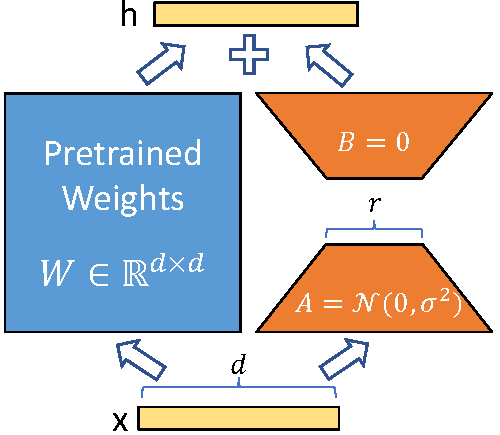
\includegraphics[width=0.29\textwidth]{images/lora.pdf}
%   \caption{LoRA}
%   \label{fig:reparam}
% \end{figure}

\subsection{Tool Integrated Reasoning}

%Tool-integrated Reasoning Agents (ToRA) \citep{Gou2024ToRA} offer a conceptual framework for augmenting large language models (LLMs) by enabling them to utilize external tools during the reasoning process. Rather than relying solely on internal language generation, ToRA integrates natural language inference with symbolic computation or code execution, treating reasoning as a hybrid process. This approach is inspired by dual-process cognitive theories—System 1 (intuitive) and System 2 (analytical)—and positions the LLM as a decision-making controller that determines when and how to delegate tasks to tools such as symbolic solvers, code interpreters, or retrieval systems.

%This paradigm is exemplified by models like AIMO2 \citep{Moshkov2025AIMO2}, which propose modular agent architectures for tool interaction, and MuMathCode \citep{Yin2024MuMathCode}, which highlights the benefits of program synthesis and iterative self-correction for improving mathematical reasoning. ToRA adopts a similar methodology, leveraging training on tool-use trajectories and imitation learning to teach models how to incorporate intermediate tool outputs into reasoning workflows. Additionally, NuminaMath \citep{Li2024NuminaMath, Fleureau2024NuminaMath} introduces symbolic memory modules that align with ToRA’s goal of maintaining coherent multi-step reasoning through persistent access to verified tool outputs.


Tool Integrated Reasoning (TIR) represents a paradigm shift in artificial intelligence systems designed for complex mathematical problem-solving. This approach addresses the inherent limitations of traditional large language models in mathematical reasoning by seamlessly combining natural language processing with external computational tools. ToRA (Tool-integrated Reasoning Agents) introduced by \citep{Gou2024ToRA}, which demonstrates how agents can leverage both analytical reasoning capabilities and specialized computational resources such as symbolic solvers and programming libraries. This integration overcomes the computational bottlenecks that have historically constrained language models when tackling advanced mathematical problems, enabling more robust and accurate problem-solving capabilities.

The effectiveness of this approach relies heavily on sophisticated training methodologies that incorporate multi-faceted data augmentation strategies.  MuMath-Code \citep{Yin2024MuMathCode}, which combines tool-enabled large language models with multi-perspective data augmentation techniques specifically for mathematical reasoning tasks. Their two-stage training approach demonstrates that integrating external Python interpreters with LLMs significantly enhances mathematical reasoning capabilities in open-source models. This methodology bridges two traditionally separate research directions in mathematical reasoning, showing that the synergy between tool utilization and data augmentation produces superior results compared to isolated approaches.

The advancement in this topic has been facilitated by the development of large-scale specialized datasets and computational resources. NuminaMath \citep{Li2024NuminaMath}, the largest public dataset in AI4Math containing 860,000 competition-level mathematical problem-solution pairs, which won the first AIMO Progress Prize. Building on such resources, \citep{Moshkov2025AIMO2} developed state-of-the-art mathematical reasoning models using the OpenMathReasoning dataset for their AIMO-2 winning solution. Additionally,  OpenCodeReasoning \citep{Ahmad2025OCRNVidia} contributed to advancing data distillation techniques for competitive programming, demonstrating the expansion of TIR applications beyond traditional mathematics into algorithmic problem-solving domains.

% Tool Integrated Reasoning enhances the reasoning capabilities of language models by integrating external tools, such as APIs or specialized algorithms, into the generation process. In the context of crime data chatbots, this approach allows the model to query real-time crime databases or perform geospatial analysis to provide users with accurate and actionable information about potential dangers.




\section{Prompting}

Basically prompting is a technique used to guide the behavior of LLMs by providing them with specific instructions or context. 
This can be done through various methods, such as zero-shot prompting, few-shot prompting, and chain-of-thought prompting. 
Each method has its own advantages and disadvantages, depending on the task at hand and the desired outcome.


\subsection{Prompt Engineering}

% https://www.promptingguide.ai/ cite from here 
Prompt engineering is an emerging field focused on crafting and refining prompts to make the most effective use of language models (LMs) 
across diverse applications and research areas. It plays a crucial role in enhancing our understanding of the strengths and limitations of LLMs. 
Beyond simply writing prompts, prompt engineering involves a broad set of techniques essential for building with, interacting with, and expanding the capabilities of LLMs. 
It also contributes to improving model safety and enables the integration of specialized knowledge and functionalities into LLM-based systems

The following methods are some of the most common techniques and used in our work:

\begin{itemize}
    \item \textbf{Zero-shot prompting}: Involves providing the model with a task description or question without any examples. The model is expected to generate a response based solely on its pre-existing knowledge and understanding of the task.
    \item \textbf{Few-shot prompting}: As mentioned by \cite{gpt3Paper}, this technique involves providing the model with a few examples of the desired output format or task. This helps the model understand the context and generate more accurate responses. A related approach is "one-shot prompting," in which the model is given only a single example.
    \item \textbf{Chain-of-thought prompting}: Firstly introduced by \cite{chainofthought2023}, encourages the model to generate intermediate reasoning steps before arriving at a final answer. This approach has been shown to improve performance on complex tasks, such as arithmetic reasoning and logical inference.
    % TODO: PAL https://www.promptingguide.ai/techniques/pal
\end{itemize}




% \section{Retrieval Augmented Generation (RAG)}

% Retrieval-Augmented Generation (RAG), first introduced by \citep{RAG2021}, is a framework that combines the strengths of retrieval-based and generative approaches for question answering. Its core idea is to enhance the generative capabilities of language models by incorporating relevant information retrieved from external knowledge sources, rather than relying solely on parametric knowledge (i.e., information encoded in the model's weights).

% The RAG architecture consists of two primary components: 
% \begin{itemize}
     
%     \item \textbf{Retriever}: This component retrieves relevant documents or sentences from a large corpus based on the input query. It typically employs models such as BM25 \citep{bm25Paper} or dense retrieval methods to identify the most relevant information. 
%     \item \textbf{Generator}: Once the retriever has collected the relevant documents, the generator—usually a transformer-based language model—takes them as input to produce a coherent and contextually appropriate response. The generator can be fine-tuned for specific tasks to further improve its performance. 
% \end{itemize}

% In recent years, RAG has gained considerable attention in the NLP community for its ability to generate high-quality responses. This has spurred the development of new techniques to improve both retrieval precision and generation quality. For instance, \citep{modularRAG2024} introduces a modular RAG framework that enables the integration of diverse components across different stages of the pipeline. These include techniques such as query expansion, reformulation, and transformation in the pre-retrieval phase, as well as the use of LLMs as judges in the post-retrieval phase to evaluate if the response is enoughly complete.
% This modular design encourages flexibility and supports experimentation with novel combinations and architectural variations.

\section{Metrics}

This section presents the evaluation metrics used to assess model performance in the context of code generation tasks. Each metric offers a different perspective on how accurately and effectively our models respond to user queries about crime data.

\subsection{Pass@K}

Pass@k is a metric that evaluates the probability of a model generating a correct answer within the top-k responses. It is particularly useful for assessing the performance of language models in tasks where multiple answers can be generated, such as question answering or text generation \citep{Levi2024SimpleModelInferenceScalingLaws}. The metric is defined as:

\begin{equation}
    Pass@k = \frac{1}{N} \sum_{i=1}^{N} \mathbb{I}(y_i \in \hat{y}_i^{(1:k)})
\end{equation}

where \(N\) is the number of samples, \(y_i\) is the ground truth answer for sample \(i\), and \(\hat{y}_i^{(1:k)}\) is the set of the top-k generated answers for sample \(i\). The indicator function \(\mathbb{I}\) returns 1 if the ground truth answer is in the top-k responses, and 0 otherwise.

% \subsection{Majority@K}

% Majority@k is a metric that evaluates if the group with the majority of the top-k generated answers is similar to the ground truth answer. It is particularly useful for assessing the performance of language models in tasks where multiple answers can be generated, such as question answering or text generation \citep{Wang2023SelfConsistency}. The metric is defined as:
% \begin{equation}
%     Majority@k = \frac{1}{N} \sum_{i=1}^{N} \mathbb{I}(y_i \in \text{majority}(\hat{y}_i^{(1:k)}))
% \end{equation}
% where \(N\) is the number of samples, \(y_i\) is the ground truth answer for sample \(i\), and \(\hat{y}_i^{(1:k)}\) is the set of the top-k generated answers for sample \(i\). The indicator function \(\mathbb{I}\) returns 1 if the ground truth answer is in the majority of the top-k responses, and 0 otherwise.


\subsection{Code-BLEU}

CodeBLEU is a specialized metric designed to evaluate the quality of code generation by comparing machine-generated code against one or more reference implementations. It extends the traditional BLEU metric \citep{Papineni2002BLEU}, commonly used in natural language processing for tasks such as machine translation—by incorporating programming-specific characteristics such as syntax, structure, and semantic correctness \citep{Ren2020CodeBLEU}. This makes CodeBLEU better aligned with the nuanced requirements of programming languages.

The metric is formulated as a weighted linear combination of four complementary components:
\begin{equation}
    \text{CodeBLEU} = \alpha \cdot \text{BLEU} + \beta \cdot \text{BLEU}_{\text{weight}} + \gamma \cdot \text{Match}_{\text{AST}} + \delta \cdot \text{Match}_{\text{DF}}
\end{equation}
Here, \(\text{BLEU}\) is the standard BLEU score, \(\text{BLEU}_{\text{weight}}\) is a weighted variant that accounts for the relative importance of different n-grams, \(\text{Match}_{\text{AST}}\) measures syntactic similarity based on abstract syntax trees (ASTs), and \(\text{Match}_{\text{DF}}\) evaluates semantic similarity through data flow analysis. The coefficients \(\alpha\), \(\beta\), \(\gamma\), and \(\delta\) are tunable hyperparameters that balance the influence of each component.

The BLEU component is computed as:

\begin{equation}
    \text{BLEU} = BP \cdot \exp\left(\sum_{n=1}^{N} w_n \cdot \log p_n\right)
\end{equation}

where \(BP\) is the brevity penalty, \(w_n\) denotes the weight assigned to n-grams of length \(n\), and \(p_n\) is the precision of those n-grams in the generated code relative to the reference code.



% \subsection{Exact Match (EM)}

% \subsection{Accuracy}

% \subsection{Precision}

% \subsection{Recall}

% \subsection{F1}

% \subsection{BERTScore}

% \subsection{Hit Rate}

% \subsection{Mean Reciprocal Rank (MRR)}


\section{Final considerations}

This chapter established the theoretical foundations necessary to understand the construction of intelligent crime data interfaces using LLMs. It first introduced spatio-temporal data as a formal structure to model real-world phenomena, particularly criminal incidents, across both time and space. It then detailed how LLMs, built on the transformer architecture, can be trained and adapted through supervised fine-tuning, instruction tuning, and parameter-efficient methods like LoRA to specialize in tasks such as answering user queries or interpreting structured crime datasets.

The chapter also explored prompting strategies and tool-integrated reasoning, which enable LLMs to go beyond static text generation to incorporate external data tools and iterative logic. Finally, it reviewed evaluation metrics such as Pass@k, Majority@k, and CodeBLEU, which are crucial for assessing the accuracy, consistency, and functional correctness of generated outputs. These concepts set the groundwork for the subsequent chapters.